\documentclass[12pt, a4paper]{article}

\usepackage{amsmath}
\usepackage{bm}
\usepackage{array}
\usepackage{amsmath}
\usepackage[portuguese]{babel}
\usepackage{chngpage}
\usepackage{float}
\usepackage[a4paper, margin=2cm]{geometry}
\usepackage{graphicx}
\usepackage{hyperref}
\usepackage{listings}
\usepackage{setspace}
\usepackage{xcolor}

\lstdefinestyle{codestyle}{
    commentstyle=\color{teal},
    keywordstyle=\color{blue},
    numberstyle=\ttfamily\color{gray},
    stringstyle=\color{red},
    basicstyle=\ttfamily\footnotesize,
    breakatwhitespace=false,
    breaklines=false,
    keepspaces=true,
    numbers=none,
    showspaces=false,
    showstringspaces=false,
    showtabs=false,
    tabsize=4
}
\lstset{style=codestyle}

\title{\Huge \textbf{Computação Gráfica \\ \Large Trabalho Prático -- Fase IV}}
\date{18 de maio de 2025}
\author{Grupo 3}

\begin{document}

\begin{center}
    
\includegraphics[width=0.25\textwidth]{res/cover/EE-C.eps}
\end{center}

\chardef\_=`_
\onehalfspacing
\setlength{\parskip}{\baselineskip}
\setlength{\parindent}{0pt}
\def\arraystretch{1.5}

{\let\newpage\relax\maketitle}
\maketitle
\thispagestyle{empty}

\vspace*{\fill}

\begin{adjustwidth}{-2cm}{-2cm} % These values only need to be large enough to center the table
    \begin{center}
        \begin{tabular}{>{\centering}p{0.25\textwidth}
                        >{\centering}p{0.25\textwidth}
                        >{\centering}p{0.25\textwidth}
                        >{\centering\arraybackslash}p{0.25\textwidth}}
            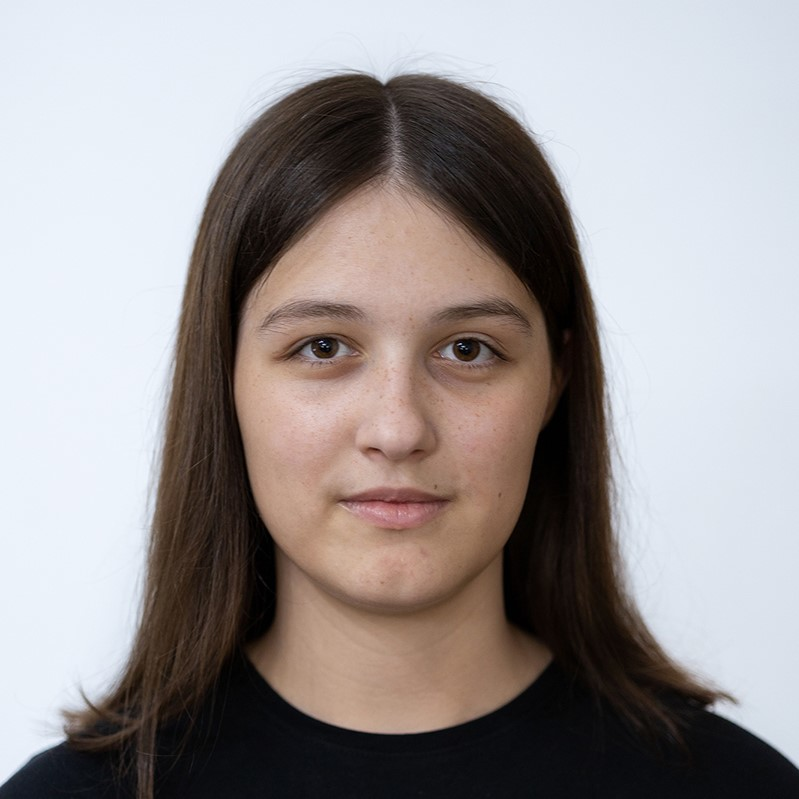
\includegraphics[width=3.5cm]{res/cover/A104437.png} &
            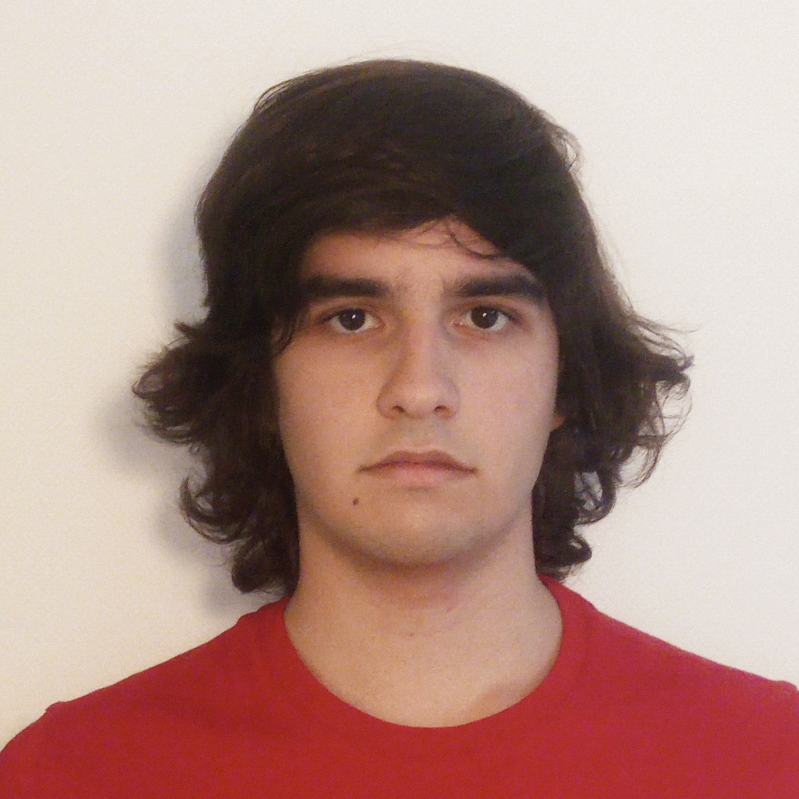
\includegraphics[width=3.5cm]{res/cover/A104348.png} &
            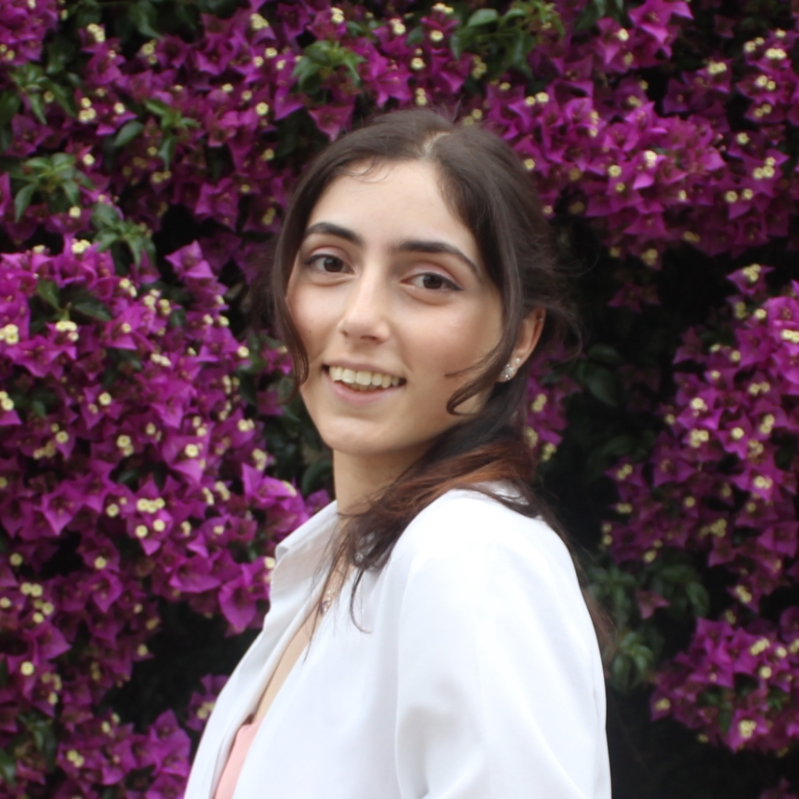
\includegraphics[width=3.5cm]{res/cover/A90817.png} &
            
\includegraphics[width=3.5cm]{res/cover/A104179.png} \\

            Ana Oliveira & Humberto Gomes & Mariana Cristino & Sara Lopes \\
            A104437      & A104348        & A90817           & A104179
        \end{tabular}
    \end{center}
\end{adjustwidth}

\pagebreak

\begin{abstract}
    \noindent
    {\color{red} TODO - Humberto}
\end{abstract}

\section{\emph{Generator}}

\subsection{Formato \texttt{.3d}}

{\color{red} TODO - Humberto}

\subsection{Plano Horizontal}

{\color{red} TODO - Humberto}

\subsection{Cubo}

{\color{red} TODO - Humberto}

\subsection{Esfera}

{\color{red} TODO - Mariana}

\subsection{Cone}

{\color{red} TODO - Ana}

\subsection{Cilindro}

{\color{red} TODO - Mariana}

\subsection{\emph{Torus}}

{\color{red} TODO - Sara}

\subsection{Outras Figuras}

{\color{red} TODO - Humberto}

\subsection{Sistema Solar}

{\color{red} TODO - Ana}

\section{\emph{Engine}}

\subsection{Geração Automática de Normais}

{\color{red} TODO - Humberto}

\subsection{Adição ao \emph{Schema} XML}

O \emph{schema} XML foi alargado para suportar materiais com múltiplas componentes de cor, texturas
e fontes de luz diversas. Estas adições permitem um controlo mais detalhado sobre o aspeto visual
dos modelos, a aplicação de texturas e a iluminação da cena.

\subsubsection{Materiais}

Pode ser associado a cada modelo um conjunto de propriedades de material que influenciam a forma
como este interage com a luz. Estas propriedades são definidas no elemento \texttt{<color>}, onde é
possível incluir as componentes \texttt{diffuse}, \texttt{ambient}, \texttt{specular} e
\texttt{emissive}, bem como o valor de \texttt{shininess}. Caso o elemento \texttt{<color>} não
esteja presente, são utilizados valores por omissão.

\begin{lstlisting}[language=xml]
<model file="sphere.3d">
    <texture file="earth.jpg" />
    <color>
        <diffuse  R="200" G="200" B="200" />
        <ambient  R="50"  G="50"  B="50"  />
        <specular R="0"   G="0"   B="0"   />
        <emissive R="0"   G="0"   B="0"   />
        <shininess value="0" />
    </color>
</model>
\end{lstlisting}

Estas propriedades são processadas na classe \texttt{Material}, que interpreta os valores a partir
do XML através de funções auxiliares definidas no módulo \texttt{XMLUtils}. O motor de renderização
utiliza depois estes parâmetros para configurar o shader correspondente.

\subsubsection{Texturas}

Caso o elemento \texttt{<texture>} esteja presente, é carregado o ficheiro de textura especificado
e aplicado ao modelo 3D. A ausência deste elemento implica que o modelo será renderizado apenas com
base nas cores definidas no material.

\begin{lstlisting}[language=xml]
<model file="cylinder.3d">
    <texture file="metal.jpg" />
</model>
\end{lstlisting}

No carregamento da cena, o caminho da textura é resolvido com base no diretório do ficheiro XML, e
a imagem é carregada para memória. O motor assegura que a mesma textura não é carregada múltiplas
vezes, reutilizando instâncias já existentes. Esta otimização é feita através de um \texttt{map}
que armazena texturas já processadas.

\subsubsection{Iluminação}

Foi também introduzido suporte para os diferentes tipos de luzes: pontuais, direcionais e
\emph{spotlights}. Todas as fontes de luz devem ser declaradas dentro do elemento \texttt{<lights>}
no ficheiro XML da cena. Cada elemento \texttt{<light>} possui um atributo \texttt{type} e
argumentos adicionais consoante o tipo de luz especificado:

\begin{itemize}
    \item \texttt{point}: requer os atributos \texttt{posX}, \texttt{posY}, \texttt{posZ} (posição);
    \item \texttt{directional}: solicita \texttt{dirX}, \texttt{dirY}, \texttt{dirZ} (direção);
    \item \texttt{spotlight}: necessita da posição, da direção e o ângulo de corte
    (\texttt{cutoff}).
\end{itemize}

\begin{lstlisting}[language=xml]
<lights>
    <light type="point"      posX="0" posY="10" posZ="0" />
    <light type="directional" dirX="1" dirY="1" dirZ="1"/>
    <light type="spotlight"  posX="0" posY="10" posZ="0"
                             dirX="1" dirY="1" dirZ="1"
                             cutoff="45" />
</lights>
\end{lstlisting}

A criação dinâmica das instâncias de luz é realizada pela \texttt{LightFactory}, com base no
atributo \texttt{type}. Cada instância herda da interface \texttt{Light}, e é posteriormente
adicionada à lista de luzes da cena.

\subsection{Texturas e Normais}

{\color{red} TODO - Humberto}

\subsection{\emph{Object Picking}}

{\color{red} TODO - Sara}

\section{Resultados Obtidos}

{\color{red} TODO - cada faz as suas prints, sem borda de janela, no tamanho especificado pela cena,
com a UI escondida (U), Humberto escreve}

\section{Conclusão}

{\color{red} TODO - Humberto}

\begingroup
\section{Bibliografia}
\renewcommand{\section}[2]{}

\begin{thebibliography}{9}
\end{thebibliography}
\endgroup

\end{document}
